% D.15 平行四边形 ABCD，E、F 为 AD、BC 中点，BE、DF 交 AC 于 M、N
\documentclass[tikz,border=4pt]{standalone}
\usepackage{ctex}
\usepackage{amsmath}
\usetikzlibrary{calc}
\begin{document}
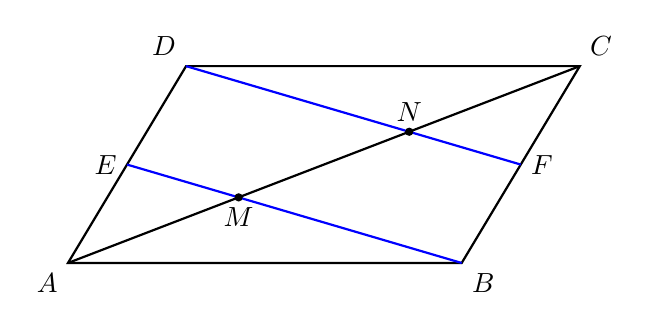
\begin{tikzpicture}[scale=1.0, thick]
  \coordinate (A) at (0, 0);
  \coordinate (B) at (5, 0);
  \coordinate (C) at (6.5, 2.5);
  \coordinate (D) at (1.5, 2.5);
  \coordinate (E) at ($(A)!0.5!(D)$);
  \coordinate (F) at ($(B)!0.5!(C)$);

  \draw (A) -- (B) -- (C) -- (D) -- cycle;
  \draw (A) -- (C);
  \draw[blue] (B) -- (E);
  \draw[blue] (D) -- (F);

  \coordinate (M) at (intersection of B--E and A--C);
  \coordinate (N) at (intersection of D--F and A--C);
  \fill (M) circle (1.5pt);
  \fill (N) circle (1.5pt);

  \node[below left]  at (A) {$A$};
  \node[below right] at (B) {$B$};
  \node[above right] at (C) {$C$};
  \node[above left]  at (D) {$D$};
  \node[left]        at (E) {$E$};
  \node[right]       at (F) {$F$};
  \node[below]       at (M) {$M$};
  \node[above]       at (N) {$N$};
\end{tikzpicture}
\end{document}
